\chapter{RESULTS \& DISCUSSIONS}

\paragraph\
This chapter presents the working system, using screenshots captured automatically by the end-to-end tests, and checks the results against the objectives in Table \ref{tab:objectives}. No accuracy figures against hiring ground truth are reported: the Kaggle dataset has category labels but no hiring outcomes, so any such figure would be invented.

\section{System walkthrough}

\begin{figure}[H]\centering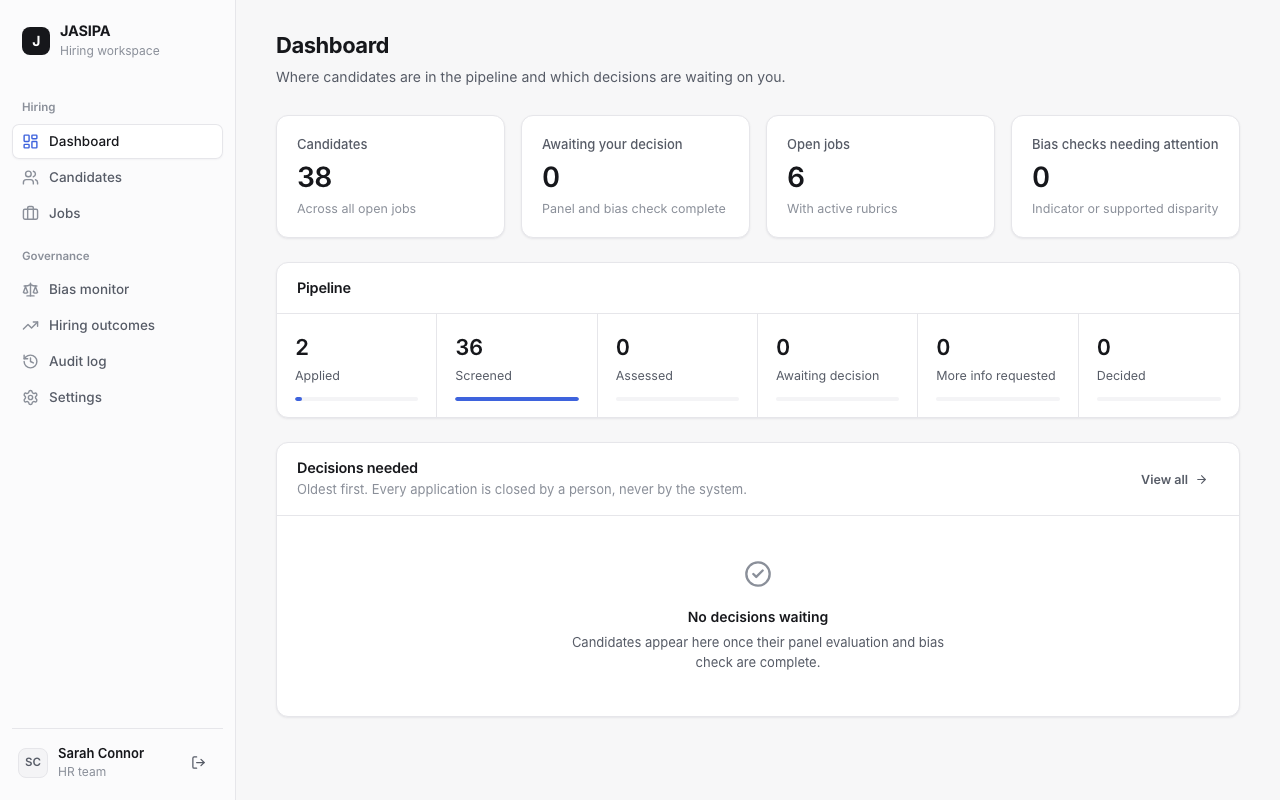
\includegraphics[width=0.92\textwidth]{../screenshots/02-dashboard.png}
\caption{HR dashboard after the Kaggle import}\label{fig:ss-dashboard}\end{figure}

\begin{figure}[H]\centering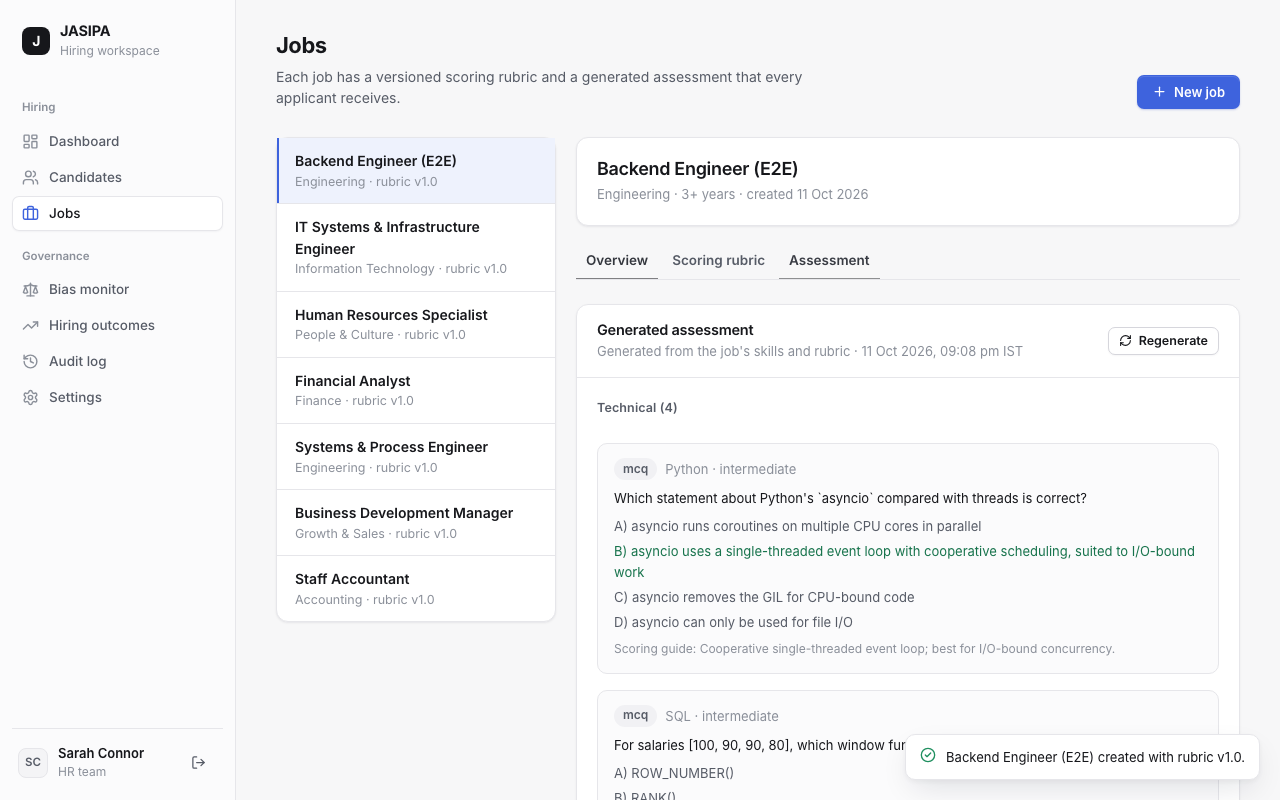
\includegraphics[width=0.92\textwidth]{../screenshots/03-job-assessment.png}
\caption{Job assessment preview generated for a Python/SQL role (MCQ, coding, scenario and STAR questions)}\label{fig:ss-job}\end{figure}

\begin{figure}[H]\centering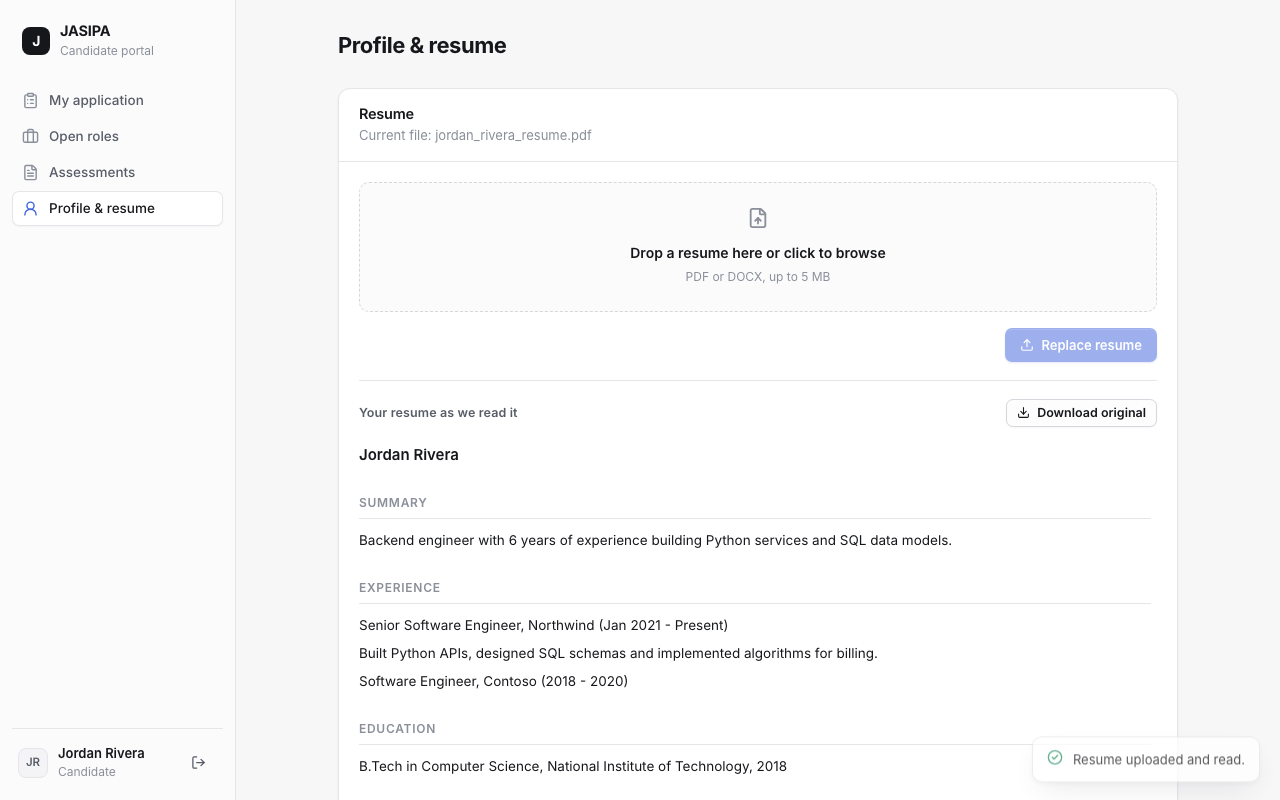
\includegraphics[width=0.92\textwidth]{../screenshots/04-candidate-resume.png}
\caption{Candidate portal: uploaded PDF resume shown in its original sections, with a download link}\label{fig:ss-resume}\end{figure}

\begin{figure}[H]\centering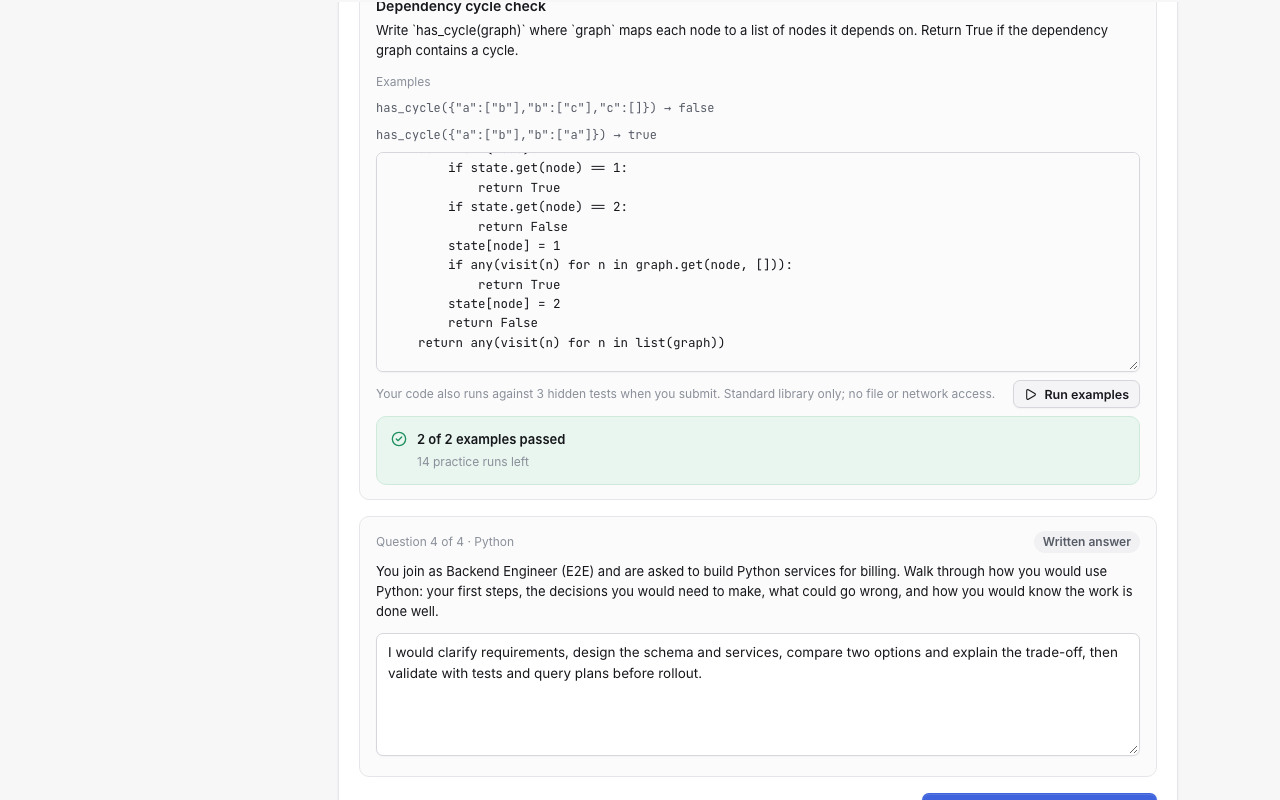
\includegraphics[width=0.92\textwidth]{../screenshots/05-candidate-coding.png}
\caption{Coding question with examples run in the sandbox}\label{fig:ss-coding}\end{figure}

\begin{figure}[H]\centering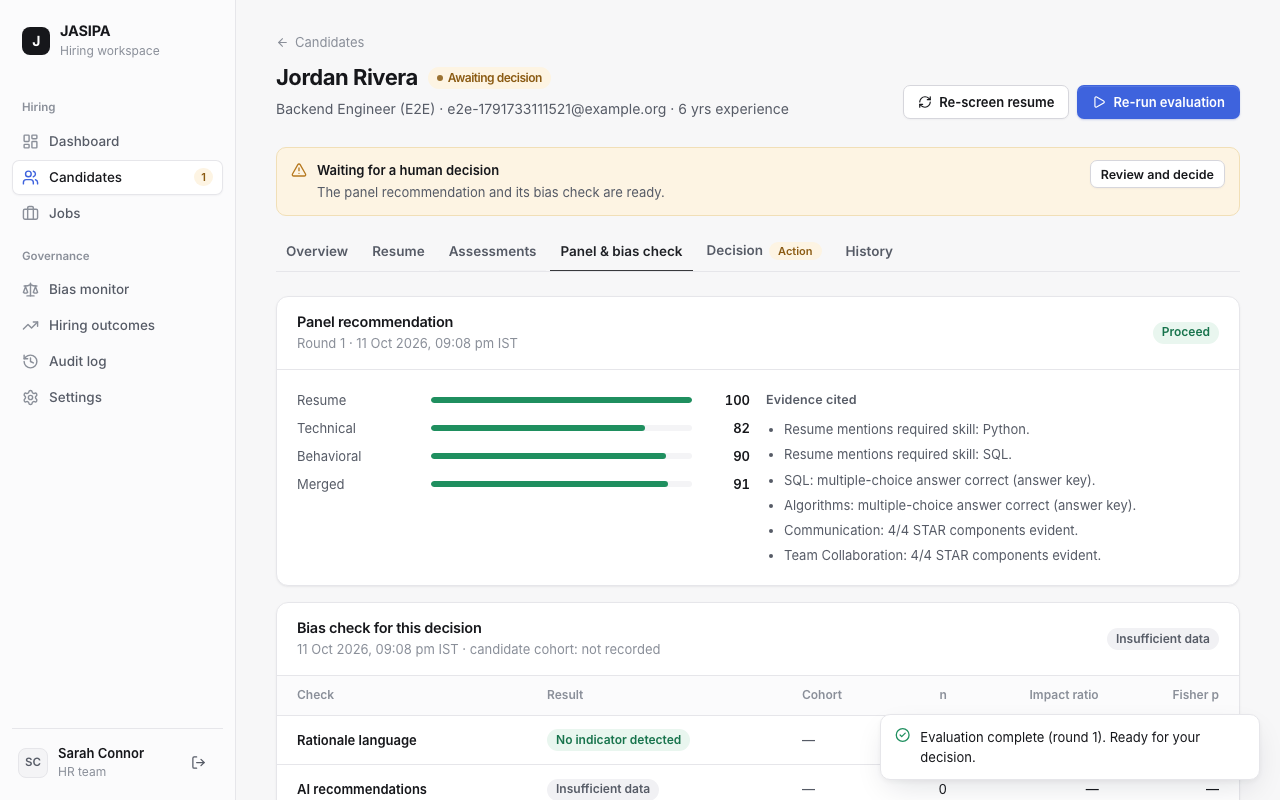
\includegraphics[width=0.92\textwidth]{../screenshots/06-panel-bias.png}
\caption{Panel recommendation and bias check: one row per check with cohort, n, impact ratio and Fisher $p$}\label{fig:ss-bias}\end{figure}

\begin{figure}[H]\centering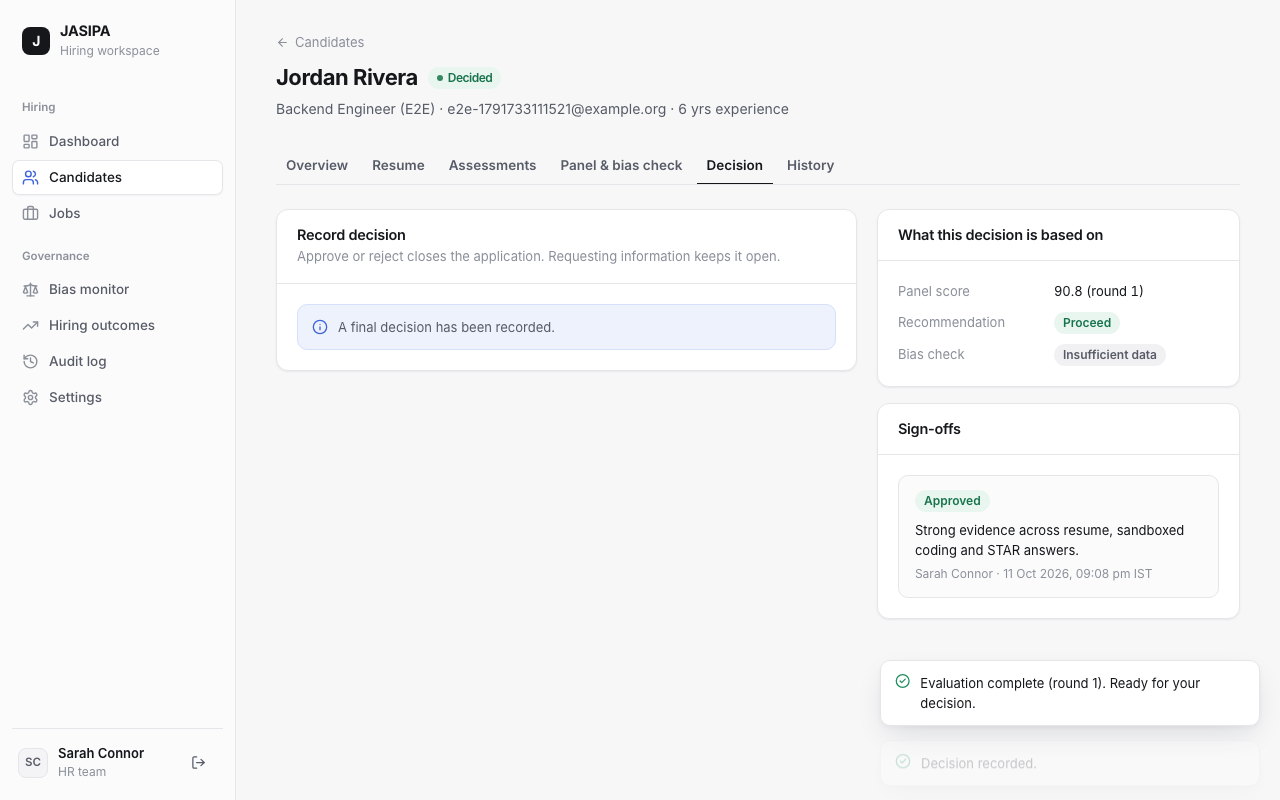
\includegraphics[width=0.92\textwidth]{../screenshots/07-decision.png}
\caption{Human decision bound to the panel decision and its bias check}\label{fig:ss-decision}\end{figure}

\begin{figure}[H]\centering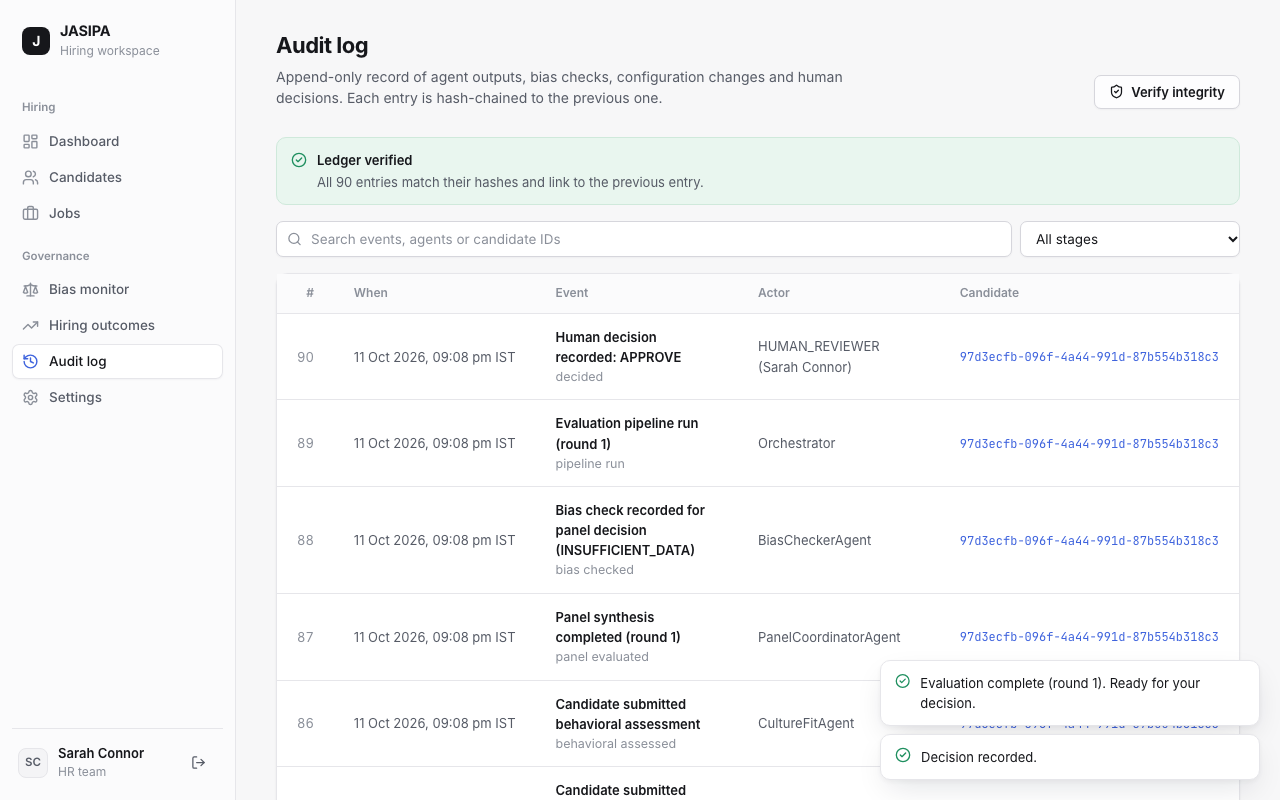
\includegraphics[width=0.92\textwidth]{../screenshots/08-audit.png}
\caption{Hash-chained audit log with integrity verification}\label{fig:ss-audit}\end{figure}

\section{Discussion}
\paragraph\
\textbf{End-to-end behaviour.} In E2E-007, a candidate who registered, uploaded a PDF resume, passed the sandboxed coding examples and submitted both assessments was evaluated by the three agents in parallel. The coordinator produced a routing label and the bias check was recorded against that panel decision. The decision page accepted the reviewer's decision only with both identifiers bound, and the audit chain verified afterwards.

\textbf{Dataset records.} The 48 imported Kaggle resumes are displayed in their original sections and are clearly marked as dataset records (Figure \ref{fig:ss-dataset} in the Appendix). They have no assessments, so a pipeline run on them returns \emph{additional information required}. This is the correct result: the system does not invent answers to complete the evidence.

\textbf{Bias check.} Because neither the Kaggle data nor the demo data contains cohort labels, the bias monitor reports \emph{Insufficient data} and shows the number of candidates excluded for missing cohorts (Figure \ref{fig:ss-monitor}). The disparity and no-indicator paths were verified with controlled cohort tables in \texttt{test\_bias}, including cases where significance and the four-fifths screen disagree. With the minimum group size of 5 and typical cohort sizes below 30, statistical power is low; the interface therefore states that \emph{not significant} does not mean \emph{no bias}.

\textbf{Regeneration.} Each successful regeneration produced a set whose fingerprint differs from the previous one, and the interface reports how many questions changed. When no different set can be produced, the API returns an error and the interface keeps the current set; it no longer reports success falsely.

\section{Validation against objectives}
\paragraph\
Objectives O1--O8 are met and each is backed by passing tests (Table \ref{tab:objectives}). Objective O5 is met in mechanism but has been validated only on controlled test data, because real cohort data was not available. Objective O9 (learning) was not implemented; Section \ref{sec:learning} explains why and what exists instead.
